\section{Evalutation}\label{sec:evaluation}

In this section, we compare the performance of state-of-the-art neural network accelerator designs and try to evaluate the techniques mentiond in section~\ref{sec:software} and section~\ref{sec:hardware}. The designs used for comparison are listed in Table~\ref{tab:hardware_list}. For data format, the "INT A/B" means that neurons are A-bit fixed point data and weights are B-bit fixed point data. We also investigate the resource utilization and draw advices to both accelerator designers and FPGA manufacturers.

\begin{table}[htbp]
    \centering
    \caption{Performance and resource utilization of state-of-the-art neural network accelerator designs}
    \begin{tabular}{r|c|c|c|c|ccc|c}
        \toprule
        \multicolumn{1}{c|}{} & Data  & Speed & Power & Eff. & \multicolumn{3}{c|}{Resource(\%)} & \multirow{2}[4]{*}{FPGA chip} \\ %\cline{6-8}
        \multicolumn{1}{c|}{} & Format & (GOP/s) & (W)   & (GOP/J) & DSP   & logic & BRAM  &  \\
        \hline
            \cite{nakahara2017fully}    & 1bit      & 329.47    & 2.3   & 143.2 & 1     & 34    & 11    & Zynq XC7Z020 \\ 
            \cite{moss2017high}         & 1bit      & 40770     & 48    & 849.38 &   -   &   -   &   -   & GX1155 \\ 
            \cite{jiao2017accelerating} & 2bit      & 410.22    & 2.26  & 181.51 & 41   & 83    & 38    & Zynq XC7Z020 \\ 
            \cite{guo2017angel}         & INT8      & 84.3      & 3.5   & 24.1  & 87    & 84    & 89    & XC7Z020 \\ 
            \cite{suda2016throughput}   & INT16/8   & 117.8     & 19.1  & 6.2   & 13    & 22    & 65    & 5SGSD8 \\ 
            \cite{liu2016automatic}     & INT16/8   & 222.1     & 24.8  & 8.96  & 40    & 27    & 40    & XC7VX690T \\ 
            \cite{ma2017optimizing}     & INT16/8   & 645.25    & 21.2  & 30.43 & 100   & 38    & 70    & GX1150 \\             
            \cite{han2017ese}           & INT16/12  & 2520      & 41    & 61.5  & 54    & 89    & 88    & XCKU060 \\ 
            \cite{venieris2017fpgaconvnet} & INT16  & 12.73     & 1.75  & 7.27  & 95    & 67    & 6     & XC7Z020 \\ 
            \cite{qiu2016going}         & INT16     & 136.97    & 9.63  & 14.22 & 89    & 84    & 87    & XC7Z045 \\ 
            \cite{xiao2017exploring}    & INT16     & 229.5     & 9.4   & 24.42 & 92    & 71    & 83    & XC7Z045 \\ 
            \cite{zhang2016caffeine}    & INT16     & 354       & 26    & 13.6  & 78    & 81    & 42    & XC7VX690T \\ 
            \cite{guan2017fp}           & INT16     & 364.4     & 25    & 14.6  & 65    & 25    & 46    & 5SGSMD5 \\ 
            \cite{li2016high}           & INT16     & 565.94    & 30.2  & 22.15 & 60    & 63    & 65    & XC7VX690T \\ 
            \multirow{2}[2]{*}{\cite{Shen2018Towards}} & \multirow{2}[2]{*}{INT16} & 431  & 25 & 17.1  & 42 & 56 & 52    & XC7VX690T \\ %\cline{3-9}    
             &  & 785 & 26 & 30.2 & 53 & 8.3  & 30 & XCVU440 \\ %\hline
            \multirow{2}[2]{*}{\cite{zhang2016energy}} & \multirow{2}[0]{*}{INT16} & \multirow{2}[0]{*}{1280.3} & \multirow{2}[0]{*}{160} & \multirow{2}[0]{*}{8} & \multirow{2}[0]{*}{-} & \multirow{2}[0]{*}{-} & \multirow{2}[0]{*}{-} & XC7Z020+ \\
            &       &       &       &       &       &       &       & XC7VX690T$\times$6 \\ %\hline
            \cite{zhang2017improving}   & INT16     & 1790      & 37.46 & 47.8  & 91    & 43    & 53    & GX1150 \\ %\hline
            \cite{lu2017evaluating}     & INT16     & 2940.7    & 23.6  & 124.6 &   -   &   -   &   -   & ZCU102 \\ %\hline
            \cite{aydonat2017opencl}    & FP16      & 1382      & 45    & 30.7  & 97    & 58    & 92    & GX1150 \\ %\hline
            \cite{podili2017fast}       & INT32     & 229       & 8.04  & 28.5  & 100   & 84    & 18    & Stratix V \\ %\hline            
            \cite{guan2017fpga}         & FP32      & 7.26      & 19.63 & 0.37  & 42    & 65    & 52    & XC7VX485T \\ %\hline
            \cite{zhang2015optimizing}  & FP32      & 61.62     & 18.61 & 3.3   & 80    & 61    & 50    & XC7VX485T \\ %\hline
            \cite{zhang2017frequency}   & FP32      & 123.5     & 13.18 & 9.37  & 88    & 85    & 64    & Stratix V \\ %\hline
            \cite{zhang2017improving}   & FP32      & 866       & 41.73 & 20.75 & 87    & -     & 46    & GX1150 \\ 
            \bottomrule
        \end{tabular}%
    \label{tab:hardware_list}%
  \end{table}%

\subsection{Speed, Power and Efficiency}

Each of the designs in Table~\ref{tab:hardware_list} drawn as a point in Figure~\ref{fig:efficiency}, using $log_{10}(power)$ as x coordinate and $log_{10}(speed)$ as y axis. Therefore, $y-x=log_{10}(energy\_efficiency)$. Besides the FPGA based designs, we also plot the GPU experimental results used in \cite{guo2017angel, han2017ese} as standards to measure the FPGA designs' performance.

\subsubsection{Bit-width Reduction} Among all the designs, 1-2 bit based designs show outstanding speed and energy efficiency. This shows that extremely low bitwidth is a promising solution for high performance design. As introduced in section~\ref{sec:software:quant}, 1-2 bit network models suffer from great accuracy loss, so this technique is better applied on simple tasks now. The energy efficiency is improved by about 100$times$ comapred with 32-bit floating point designs. But there is still a great gap towards the $1000\times$ improvment estimation. This shows that memory access becomes the bottleneck for 1-2 bit designs, which only scales linearly with the bit-width. INT16/8, INT16 and INT8 are commonly adopted. But the difference between these designs are not obvious. This is due to the fact that current FPGAs implement wide multipliers in DSPs like $18\times 15$ or $18\times 18$. Using a less bits for computaion will not benefit the DSPs. The double MAC technique by~\cite{nguyen2017double} serves as a solution but is not adopted in the listed designs.

\subsubsection{Fast Convolution Algorithm} Among all the 16-bit designs, \cite{lu2017evaluating} achieves the best energy efficiency and the highest speed with the help of the $6\times 6$ Winograd fast convolution, which is $1.7\times$ faster and $2.6\times$ energy efficient than the 16-bit design in \cite{zhang2017improving}. The design in \cite{zhang2017frequency} achieves $2\times$ speedup and $3\times$ energy efficiency compared with \cite{zhang2015optimizing} where both designs use 32-bit floating point data. Overall, the improvement does not match the estimation but can still reach 2-3$\times$.

\subsubsection{System Level Optimization} The overall system optimization is not well addressed in most of the work. As this is also related to the HDL design quality, we only try to evaluate the effect. Here we compare three designs\cite{zhang2016caffeine, liu2016automatic, li2016high} on the same XC7VX690T platform and try to evaluate the effect. All the three designs implement 16-bit fixed-point data format except that ~\cite{liu2016automatic} uses 8-bit for weights. No fast convolution or sparsity is utilized in any of the work. Even though, \cite{li2016high} achieves $2.5\times$ the energy efficiency of \cite{liu2016automatic}. It shows that a system level optimization has a strong effect even comparable to the usage of fast convolution algorithm. 

\subsubsection{Comparision with GPU} In general, FPGA based designs have achieved comparable energy efficiency to GPU with 10-100GOP/J. But the speed of GPUs still surpass FPGAs.Scaling up the FPGA based design is still a problem. Zhang, et al.~\cite{zhang2016energy} propose the FPGA cluster based solution using 16-bit fixed point computation. But the energy efficiency is worse than the other 16-bit fixed-point designs. 

\begin{figure}[ht]
    \centering
    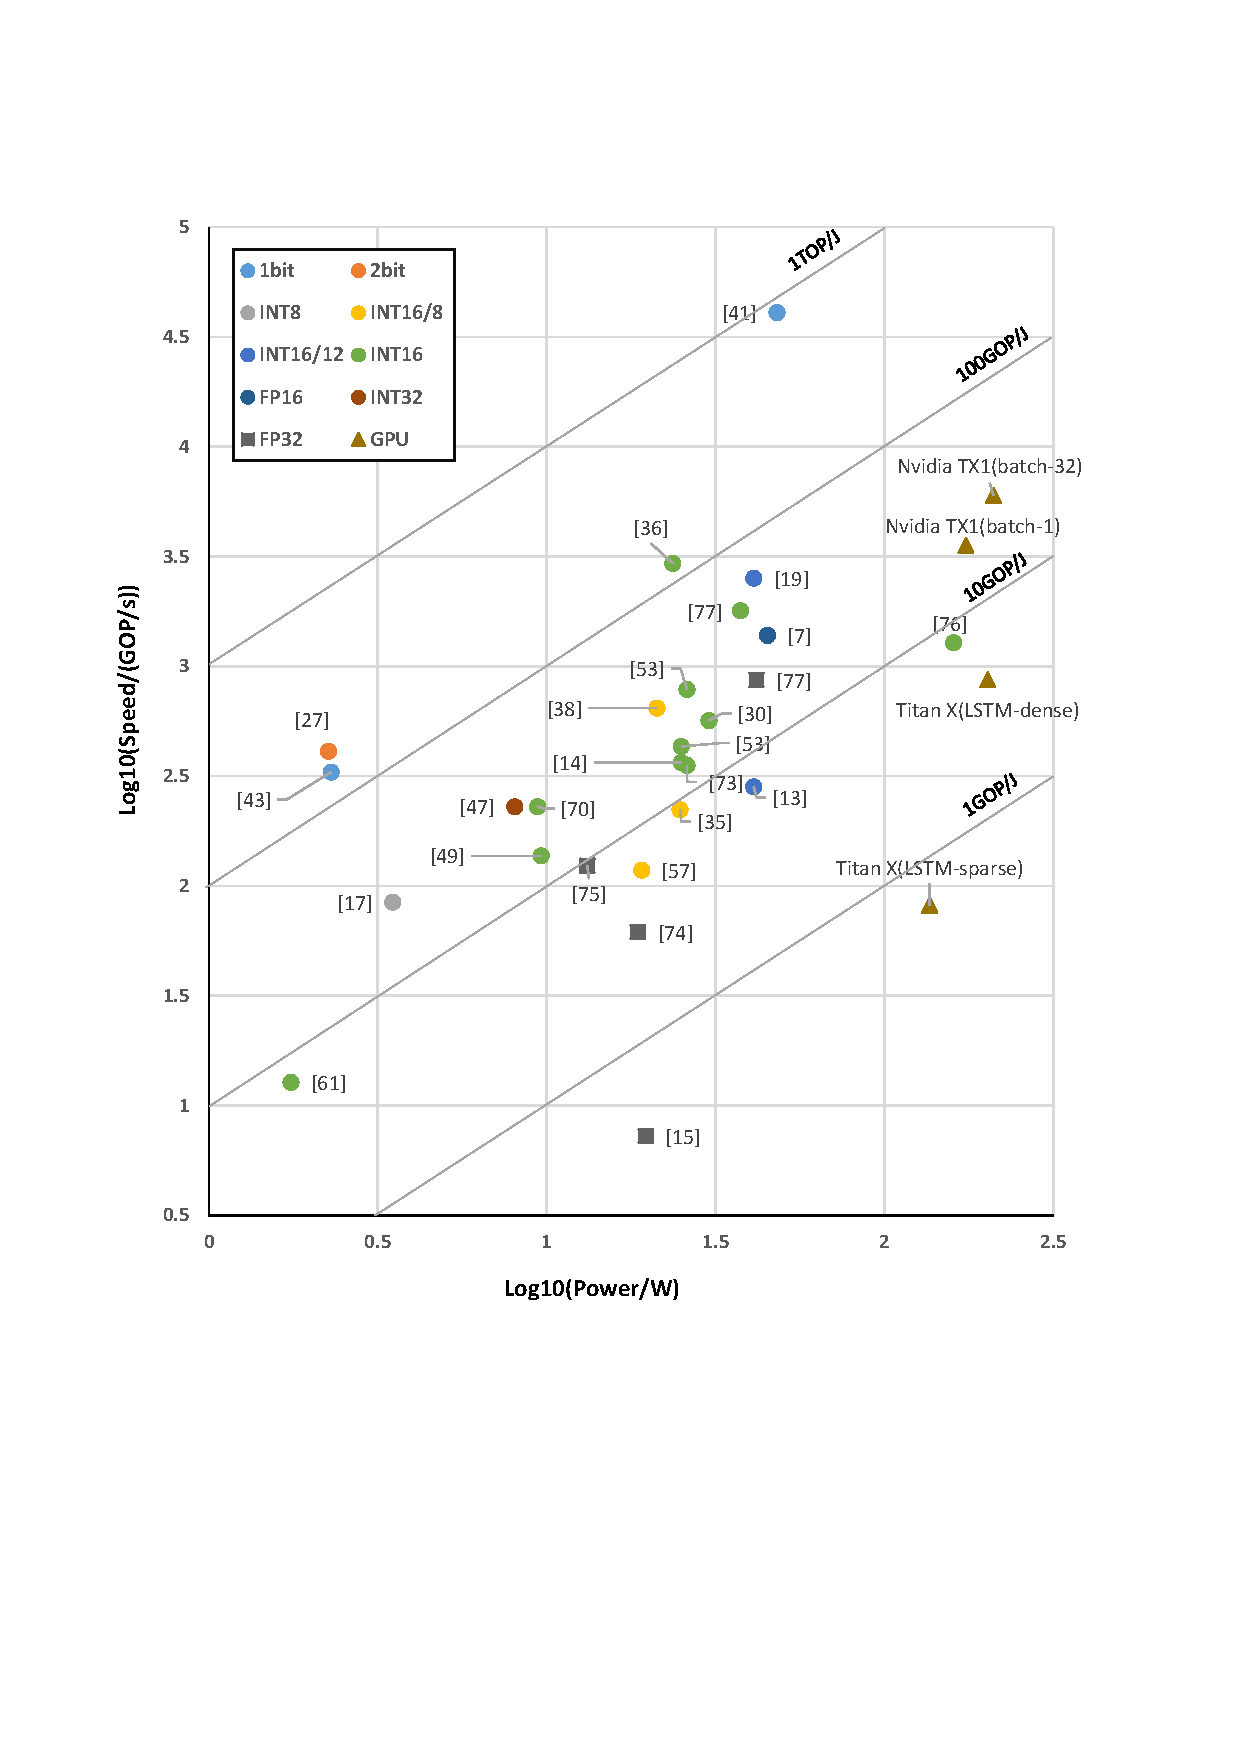
\includegraphics[width=1.0\columnwidth]{fig/efficiency.pdf}
    \caption{A comparison between different designs on a logarithm coordinate of power and performance. }
    \label{fig:efficiency}
\end{figure}

\subsection{Resource Utilization}
We also investigate the resource utilization of the designs in Table~\ref{tab:hardware_list}. Three kinds of resouce are considered, DSP, BRAM, and logic. We plot the designs in Figure~\ref{fig:resource} using two of the utilization ratio as x and y coordinate. We draw the diagonal line of each figure to show the designs' preference on hardware resource. The BRAM-DSP figure shows a obvious preference of hardware on DSP over BRAM. 

\begin{figure}[ht]
    \centering
    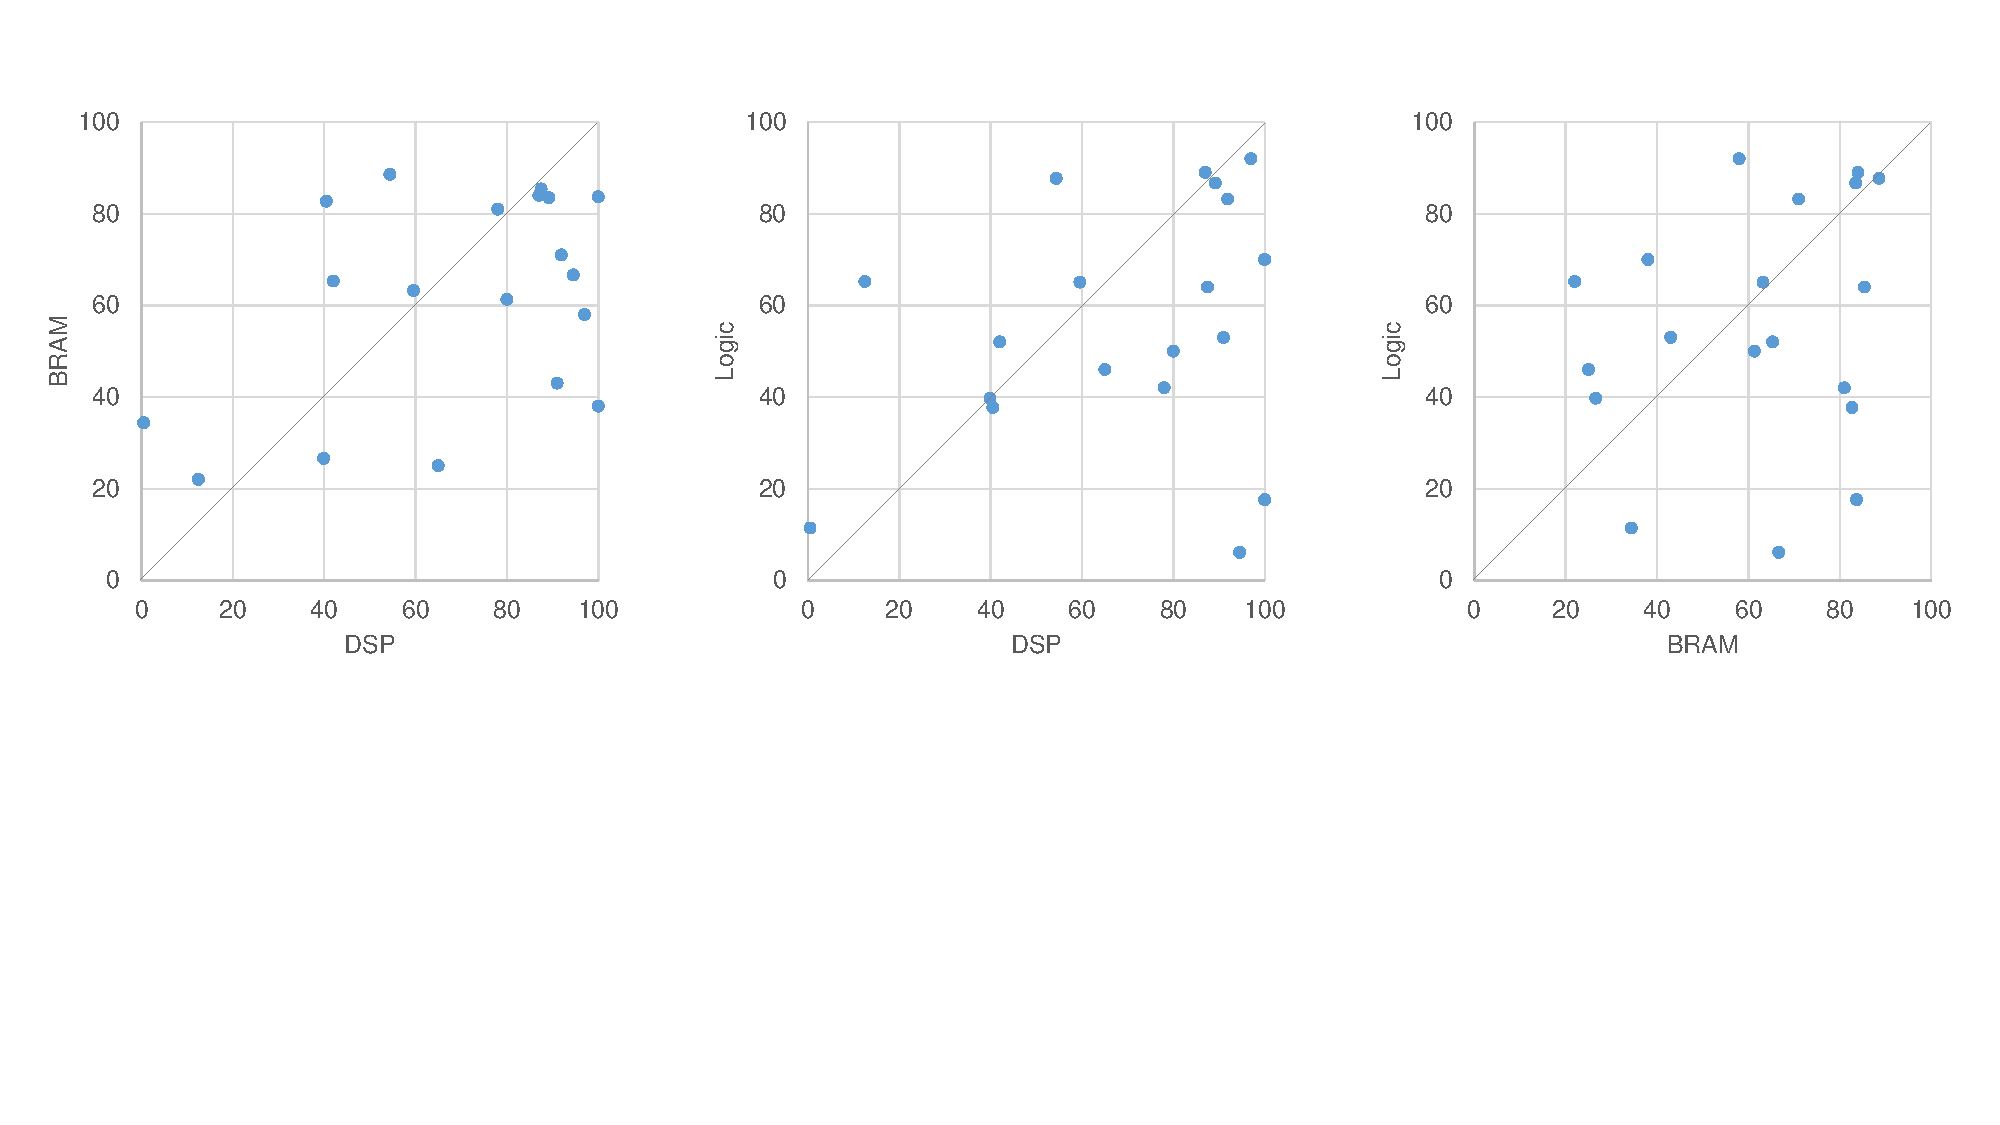
\includegraphics[width=1.0\columnwidth]{fig/resource.pdf}
    \caption{Resource utilization ratio of different accelerator designs.}
    \label{fig:resource}
\end{figure}